\section{Cache Management Using System Architecture Knowledge}
\label{sec:cache-management-using-system-archiecture-knowledge}

Using the Mantle policy engine, we test a variety of cache management tools and
algorithms on a single in-memory database node using the keyspace analysis in
Section~\S\ref{sec:parsplice-keyspace-analysis}. These strategies are
implemented as the ``when" and ``how much" policies from the Mantle API; the
``where" callback does not make sense for a single node (segments are either in
the cache or they are not). The evaluation metric is the accuracy and runtime
of each strategy; the strategy should be accurate enough so as to sacrifice
negligible performance and fast enough to run as often as we want to detect
regimes.

First we sized the cache according to our system specific knowledge. By
``system", we mean the hardware and software of the storage hierarchy. We look
at request rate, unique keys in a sliding window, and bandwidth capabilities. For
example, we know that LevelDB cannot handle high IO request rates.

% technical details
In the original ParSplice implementation, each cache node uses an unlimited
amount of memory to store segment coordinates. We limit the size of the cache
using an LRU eviction policy, where the penalty for a cache miss is retrieving
the data from the persistent database.  We evict keys (if necessary) at every
operation instead of when segments complete because the cache fills up too
quickly otherwise.

% results: cache size trade-offs
\begin{figure}[t]
  \noindent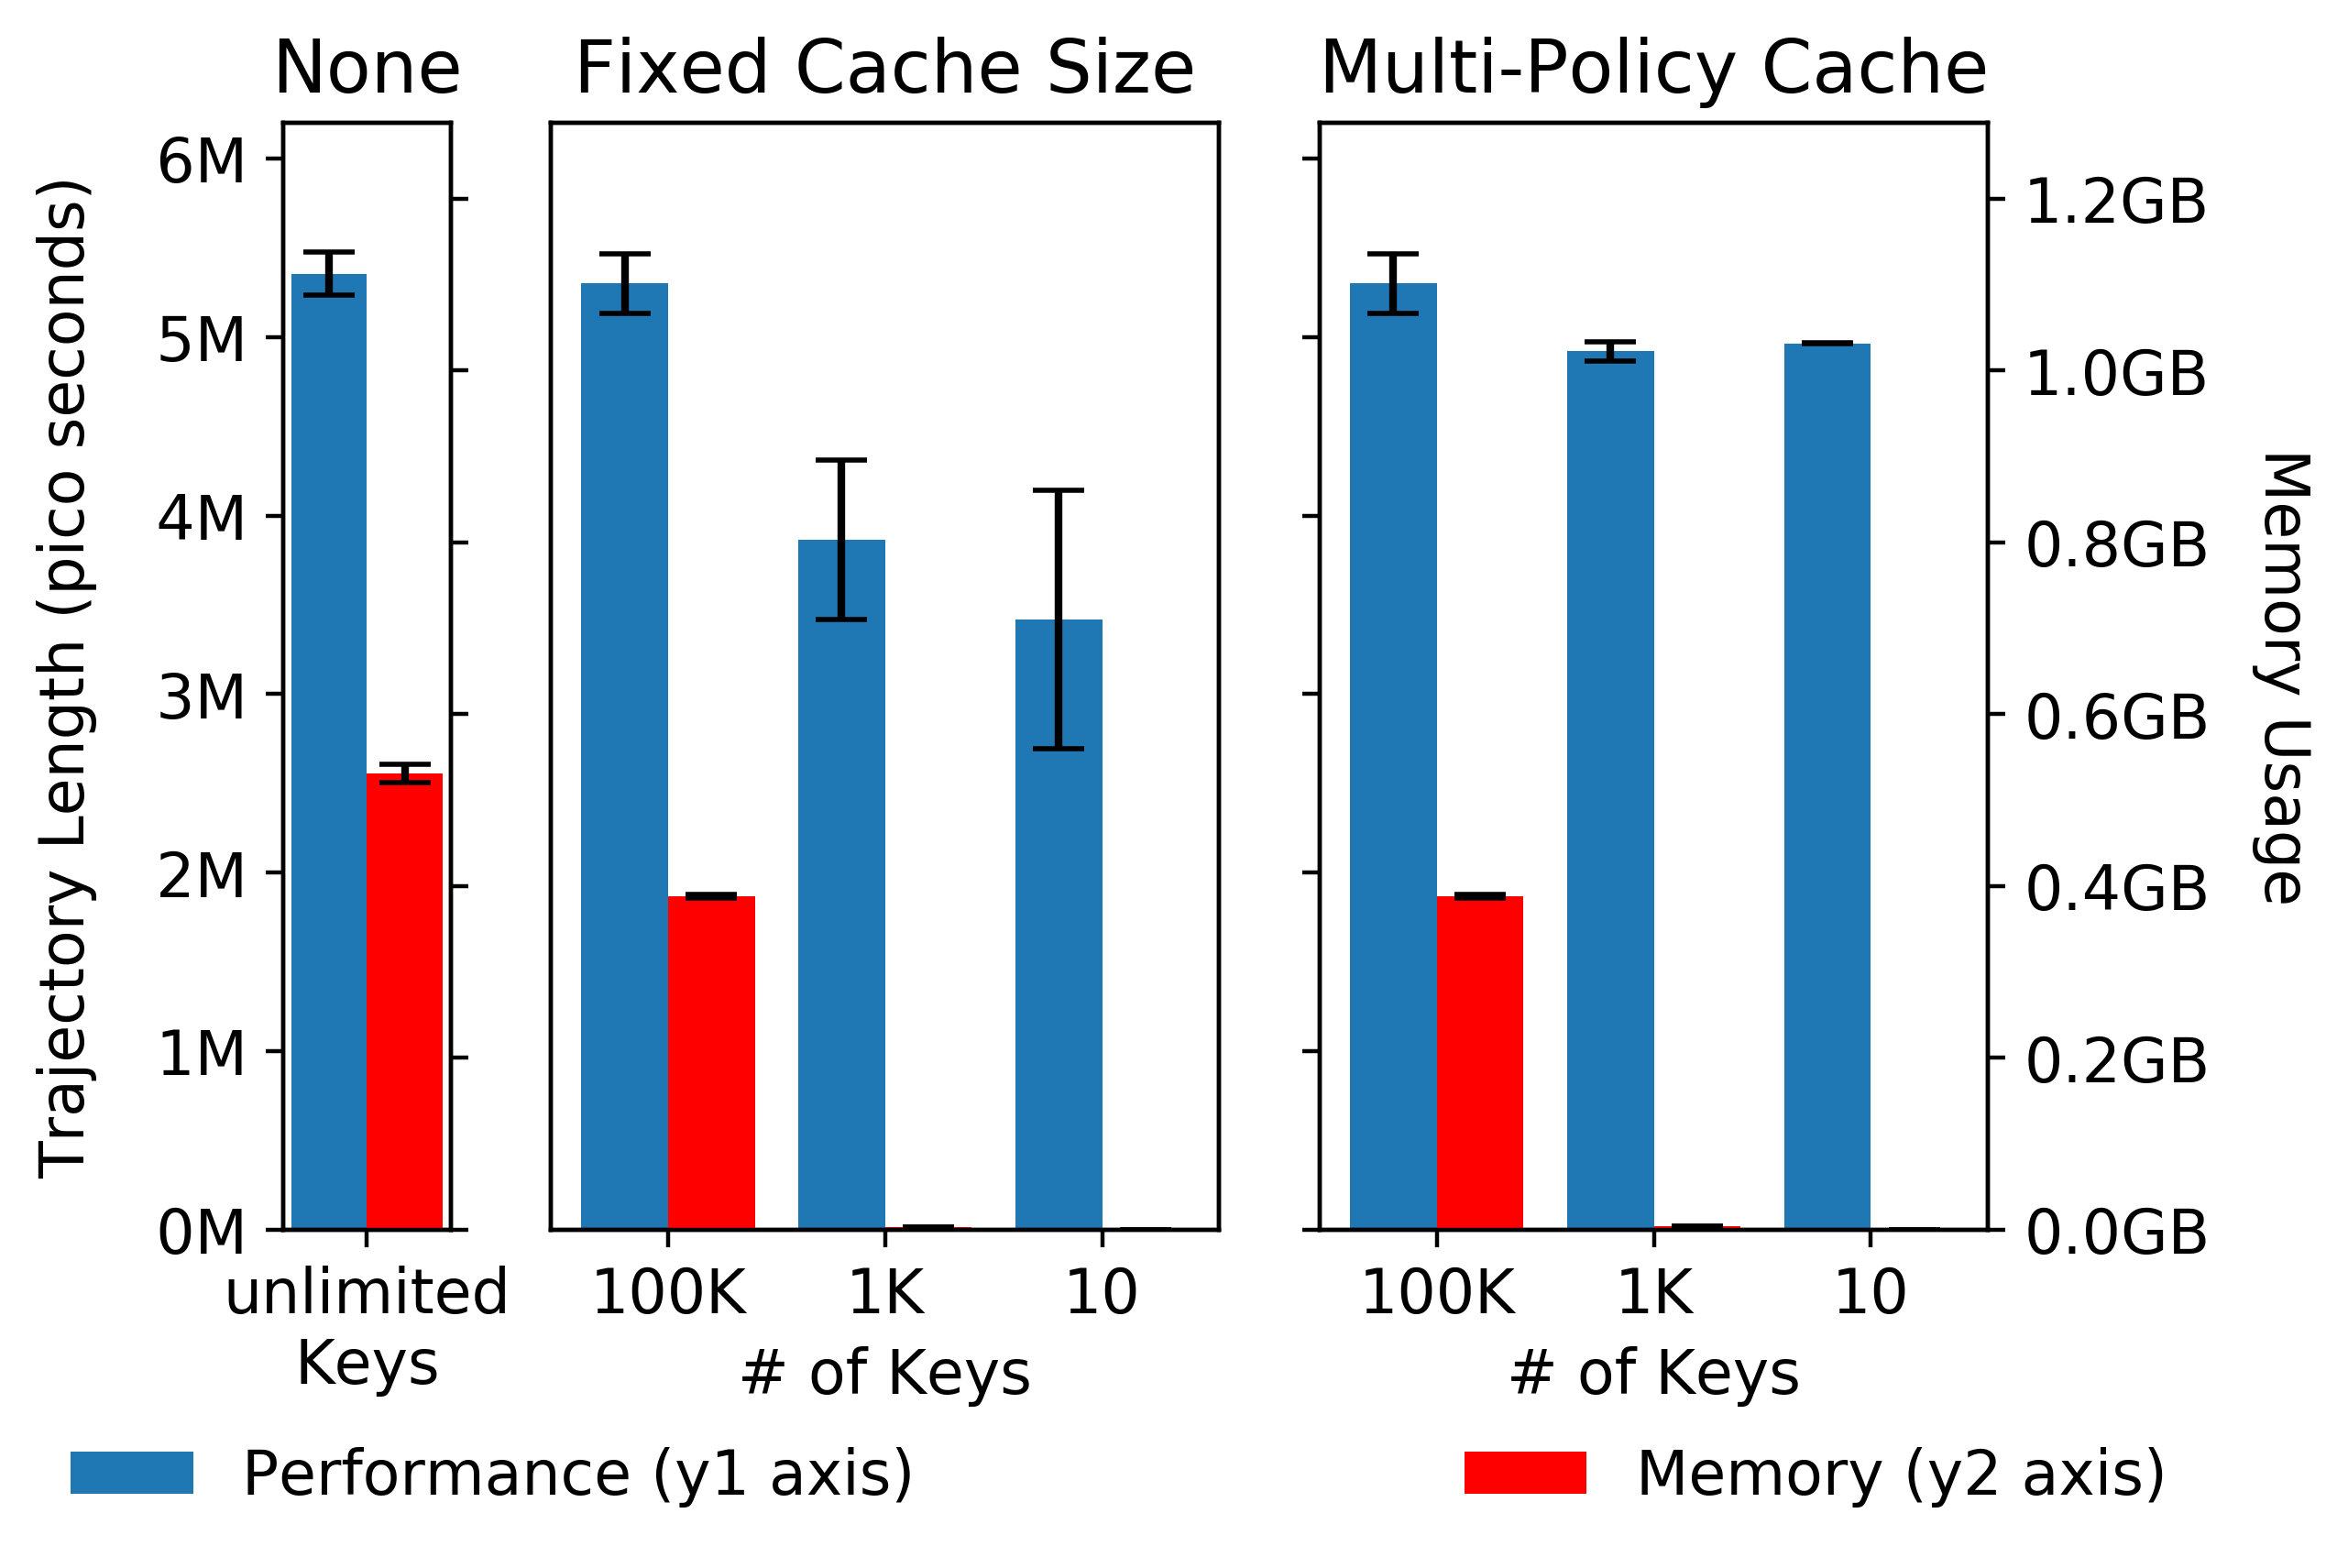
\includegraphics[width=0.5\textwidth]{figures/methodology-tradeoff.png}\\
  \caption{The performance and resource utilization trade-off for different
  cache sizes. ``Baseline" is
  ParSplice unmodified and the ``Policy: Constrain Cache Size" graph limits the
  size of the cache to save memory.  \label{fig:methodology-tradeoff}}
\end{figure}

The results for different cache sizes for a growth rate of \(\Delta_1\) over a
2.5 hour run across 256 workers is shown in
Figure~\ref{fig:methodology-tradeoff}.  ``Baseline" is the performance of
unmodified ParSplice  measured in trajectory duration (\(y\) axis) and
utilization is measured with memory footprint of just the cache (\(y2\) axis).
The other graph shares the \(y\) axis and shows the trade-off of constraining
the cache to different sizes.  The error bars are the standard deviation of 3
runs. 

% results: raw numbers
Although the keyspace grows to 150K, a 100K key cache achieves 99\% of the
performance. Decreasing the cache degrades performance and predictability.
While this result is not unexpected, it nonetheless achieves our goal of
showing the benefits of load balancing keys across nodes and that smaller
caches on each node are an effective way to save memory without completely
sacrificing performance.

% why is the performance lower for smaller caches?
Despite the memory savings, our results suggest that dynamic load balancing
policies could save even more memory.  Figure~\ref{fig:methodology-tradeoff}
show that a 100K key cache is sufficient as a static policy but the top graph
in Figure~\ref{fig:motivation-regimes} indicates that the cache size could be
much smaller. That graph shows that the beginning of the run is characterized
by many reads to a small set of keys and the end sees much lower reads per
second to a larger keyspace. Specifically, it shows only about 100 keys as
active in the latter half of the run.

After analyzing traces, we see that the 100 key cache is insufficient because
the persistent database cannot service the read-write traffic.  According to
Figure~\ref{fig:motivation-regimes}, the read requests arrive at 750 reads per
second in addition to the writes that land in each tier (about 300 puts/second,
some redundant). This traffic triggers a LevelDB compaction and reads block,
resulting in very slow progress.  Traces verify this hypothesis and show reads
getting backed up as the read/write ratio increases. To recap, small caches
incur too much load on the persistent database  at the beginning of the run but
should suffice after the initial read flash crowd passes because
the keyspace is far less active. This suggests a two-part load balancing
policy.

% Why is this a good idea
Although ParSplice does not use a distributed file system, its workload is very
similar because the minima key-value store responds to small and frequent
requests, which results in hot spots and flash crowds.  Modern distributed file
systems have found efficient ways to measure, migrate, and partition metadata
load and have shown large performance gains and
better scalability~\cite{zheng:pdsw2014-batchfs, zheng:pdsw2015-deltafs,
grider:pdsw2015-marfs, ren:sc2014-indexfs, patil:fast2011-giga+,
brandt:msst2003-lh}.  Previous work quantified the speedups achieved with
Mantle and formalized balancers that were good for file systems.

\begin{figure}[t]
  \noindent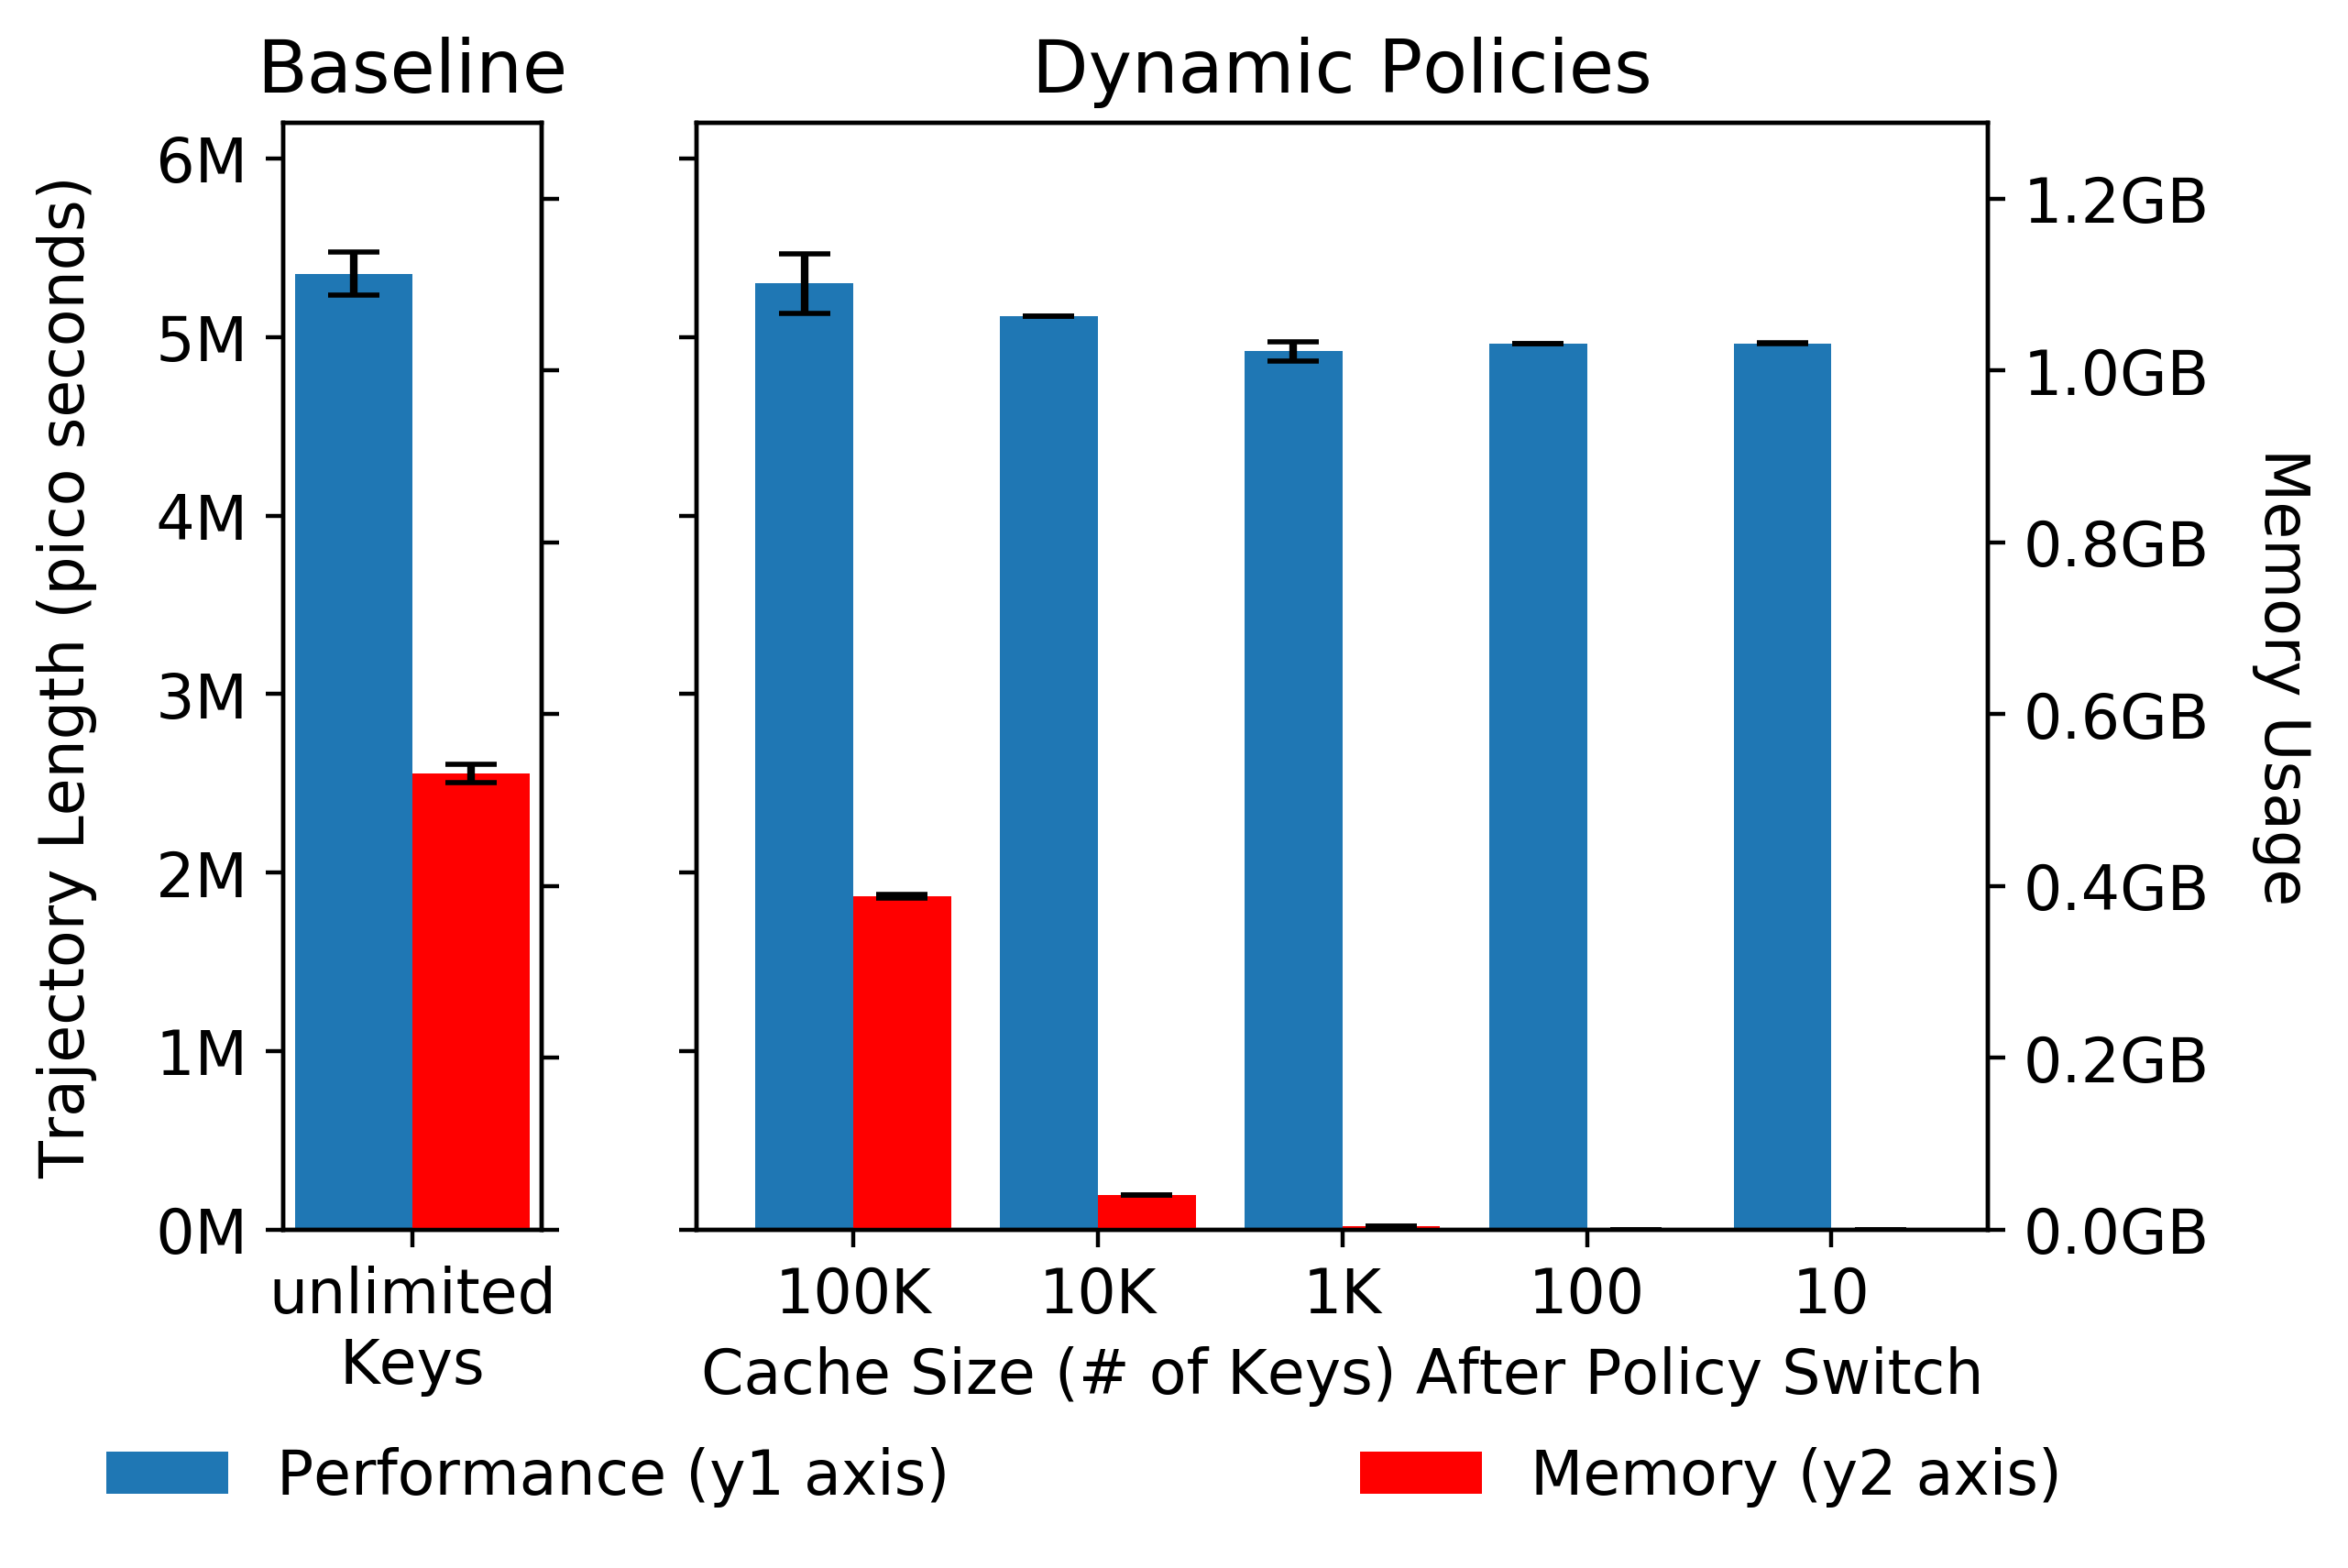
\includegraphics[width=0.5\textwidth]{figures/methodology-tradeoff-dynamic.png}\\
  \caption{The performance and resource utilization trade-off of using a
  dynamic load balancing policy that switches to a constrained cache policy after absorbing
  the initial burstiness of the workload. The sizes of these smaller caches are
  on the \(x\) axis.  \label{fig:methodology-tradeoff-dynamic}}
\end{figure}

Figure~\ref{fig:methodology-tradeoff-dynamic} shows the results of using Mantle
to program a dynamic load balancing policy into ParSplice that switches between
two policies:

\begin{itemize}
  \item unlimited growth policy: cache increases on every write
  \item \(n\) key limit policy: cache constrained to \(n\) keys
\end{itemize}

We trigger the policy switch at 100K keys to absorb the flash crowd at the
beginning of the run. Once triggered, keys are evicted to bring the size of the
cache down to the threshold.  In the bar chart, the cache sizes for the \(n\)
key limit policy are along the \(x\) axis.

% results: same level of performance can be achieved 
The dynamic policies show better performance than the single \(n\) key
policies. The performance and memory utilization for a 100K key cache size is
the same as the 100K bar in Figure~\ref{fig:methodology-tradeoff-dynamic} but
the rest reduce the size of the keyspace after the read flash crowd.  We see
the worst performance when the engine switches to the 10 key limit policy,
which achieves 94\% of the performance while only using 40KB of memory. 

% caveats: it is calculating 90% of the trajectory, memory value reported is final
\subsubsection*{Caveats}

The results in Figure~\ref{fig:methodology-tradeoff-dynamic} are slightly
deceiving for three reason: (1) segments take longer to generate later in the
run, (2) the memory footprint is the value at the end of 2.5 hours, and (3)
this policy only works well for the 2.5 hour run.  For (1), the curving down of
the simulation vs. wall-clock time is shown in
Figure~\ref{fig:methodology-trajectory}; as the nanoparticle grows it takes
longer to generate segments so by the time we reach 2 hours, over 90\% of the
trajectory is already generated.  For (2), the memory footprint is around 0.4GB
until we reach 100K key switch threshold. In
Figures~\ref{fig:methodology-tradeoff}
and~\ref{fig:methodology-tradeoff-dynamic} we plot the final value. For (3),
Figure~\ref{fig:methodology-trajectory} shows that the cache fills up with 100K
keys at time 7200 seconds and its size is reduced to the size listed in the
legend.  The curves stay close to ``Unlimited" for up to an hour after the
cache is reduced but eventually flatten out as the persistent database gets
overloaded. 10K and 100K follow the ``Unlimited" curve the longest and are
sufficient policies for the 2.5 hour runs but anything longer would need a
different dynamic load balancing policy.

\begin{figure}[t]
  \noindent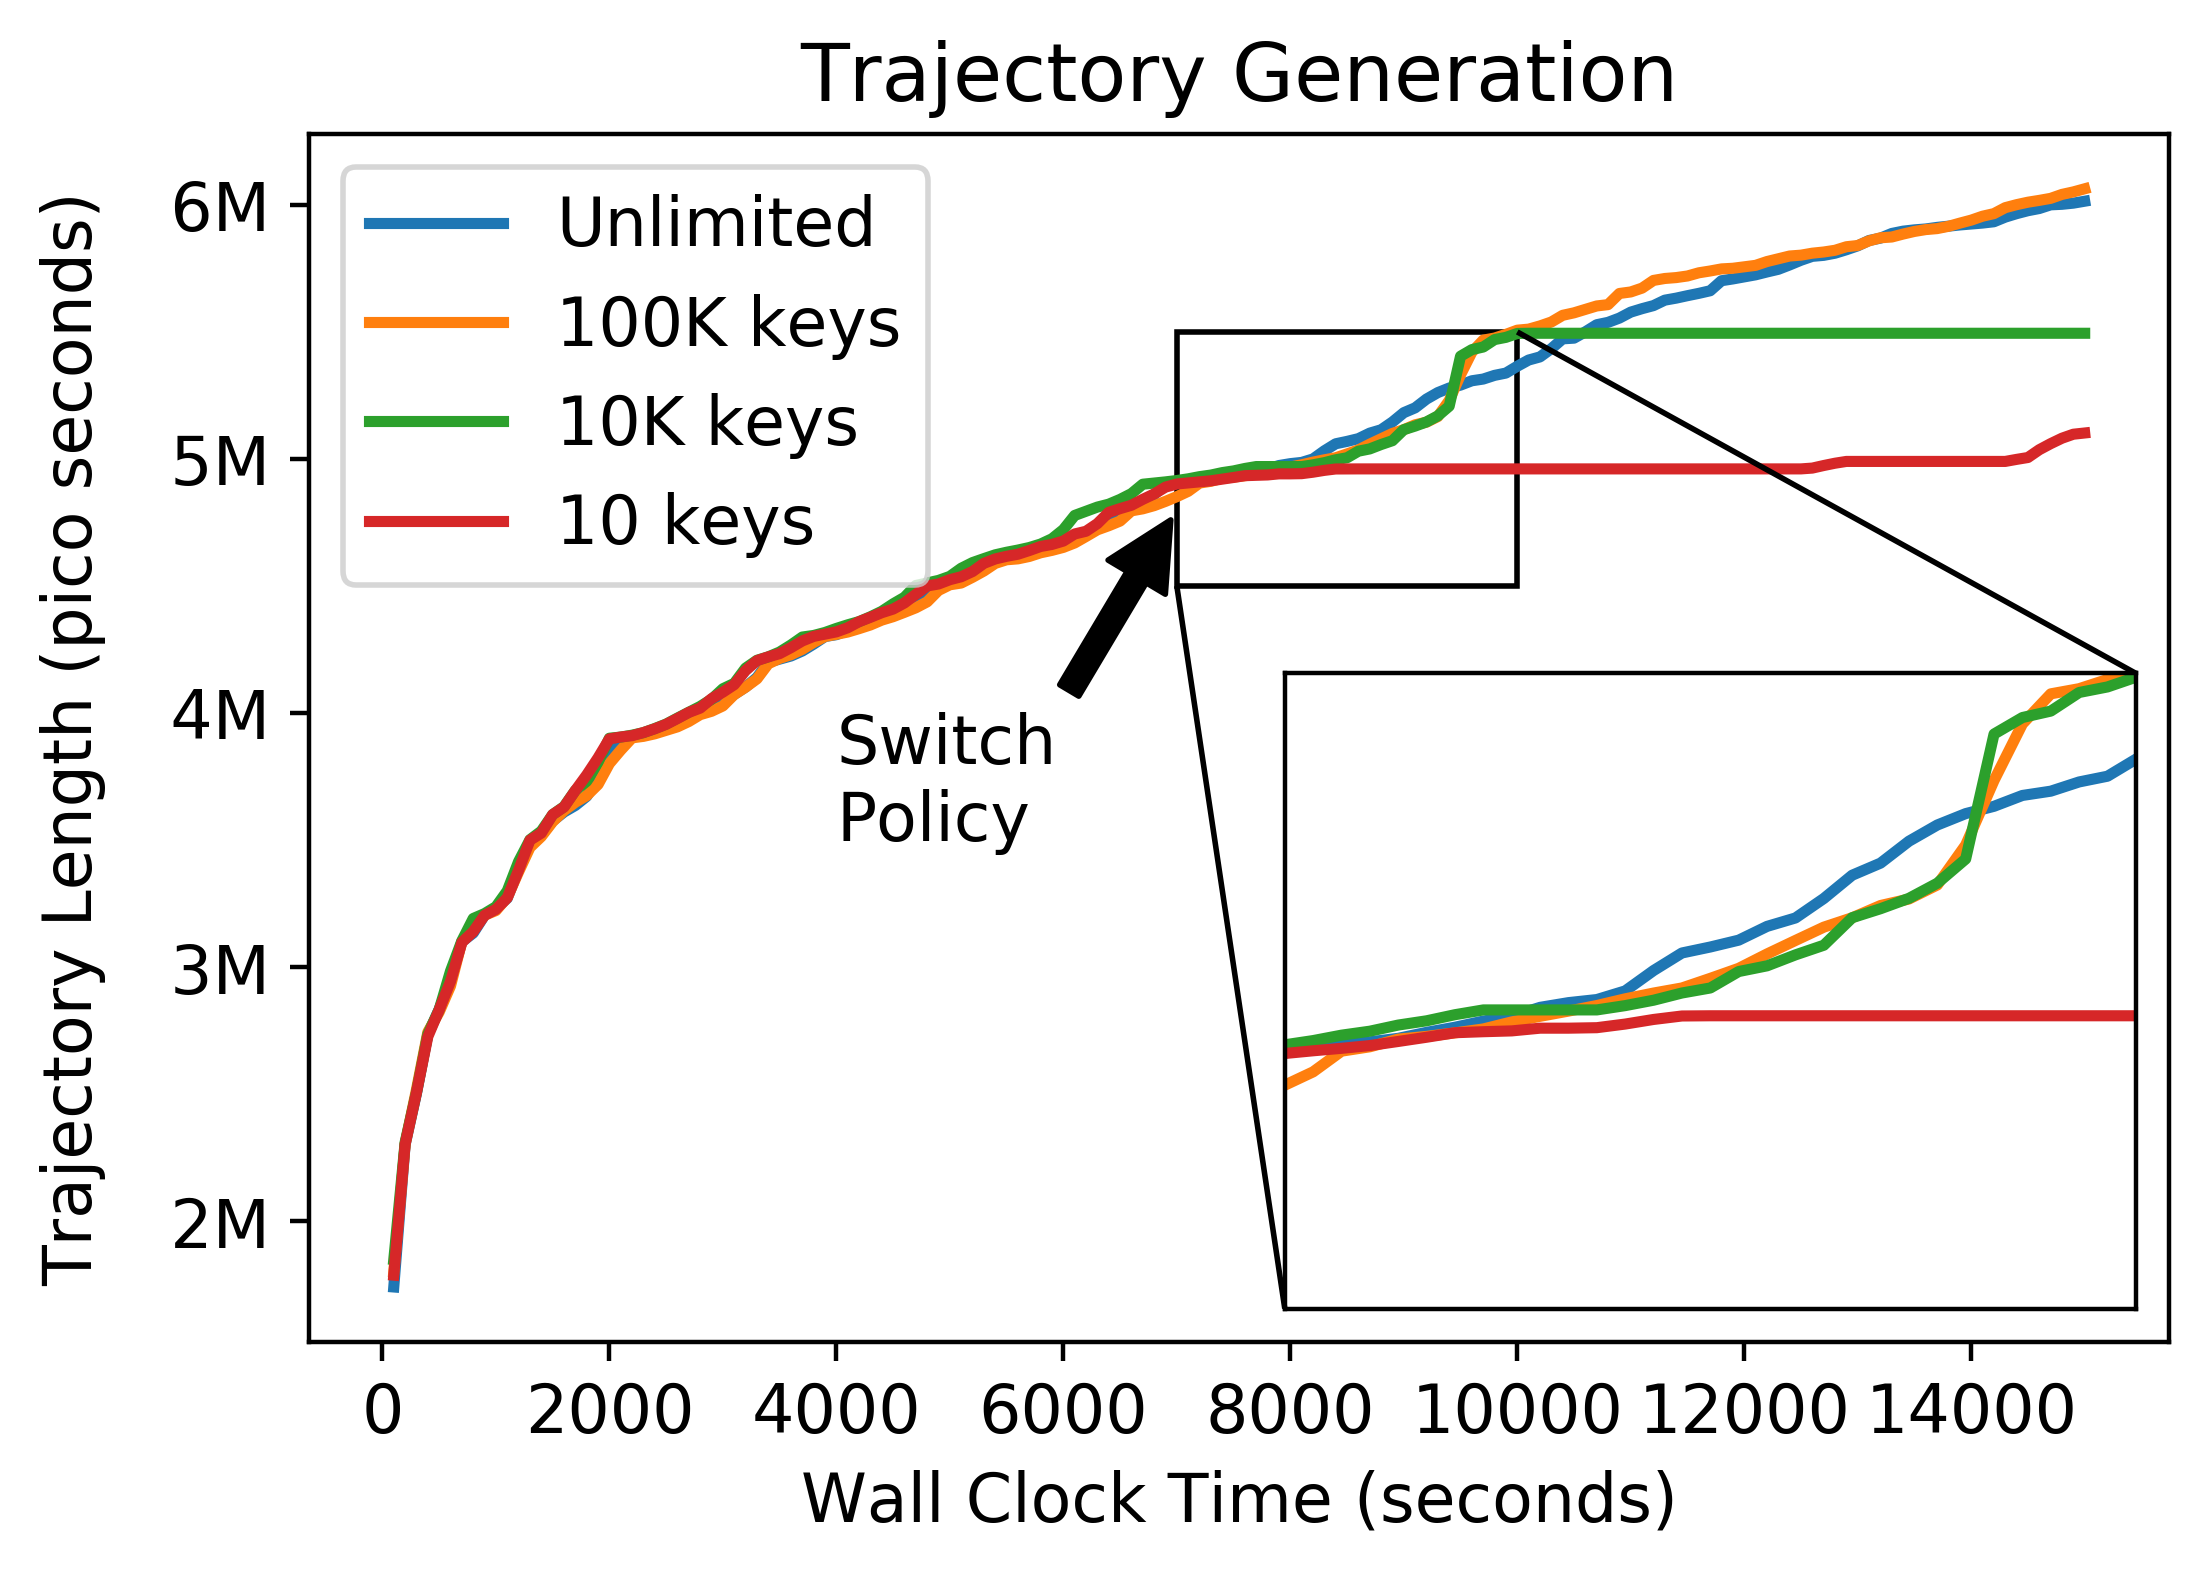
\includegraphics[height=5cm,width=0.4\textwidth]{figures/methodology-trajectory.png}\\
  \caption{The rate that the trajectory is computed decays over time (which is
  expected) but this skews the performance improvements in
  Figure~\ref{fig:methodology-tradeoff-dynamic}. Our dynamic policy works for 2.5
  hour jobs but not for 4 hour jobs.  \label{fig:methodology-trajectory}}
\end{figure}

% but the result is still valid
Despite these caveats, the result is still valid: we found a dynamic load
balancing policy that absorbs the cost of a high read throughput on a small
keyspace and reduces the memory pressure for a 2.5 hour run. Our experiments
show the effectiveness of the load balancing policy engine we integrated into
ParSplice, not that we were able to identify the best policy for all system
setups ({\it i.e.} different ParSplice parameters, number of worker tasks, and
job lengths).  To solve that problem, we need a way to identify what thresholds
we should use for different job permutations.

\section{Cache Management Using Domain-Specific Application Knowledge}
\label{sec:cache-management-using-domain-specific-knowledge}
\begin{figure}[t]
  \noindent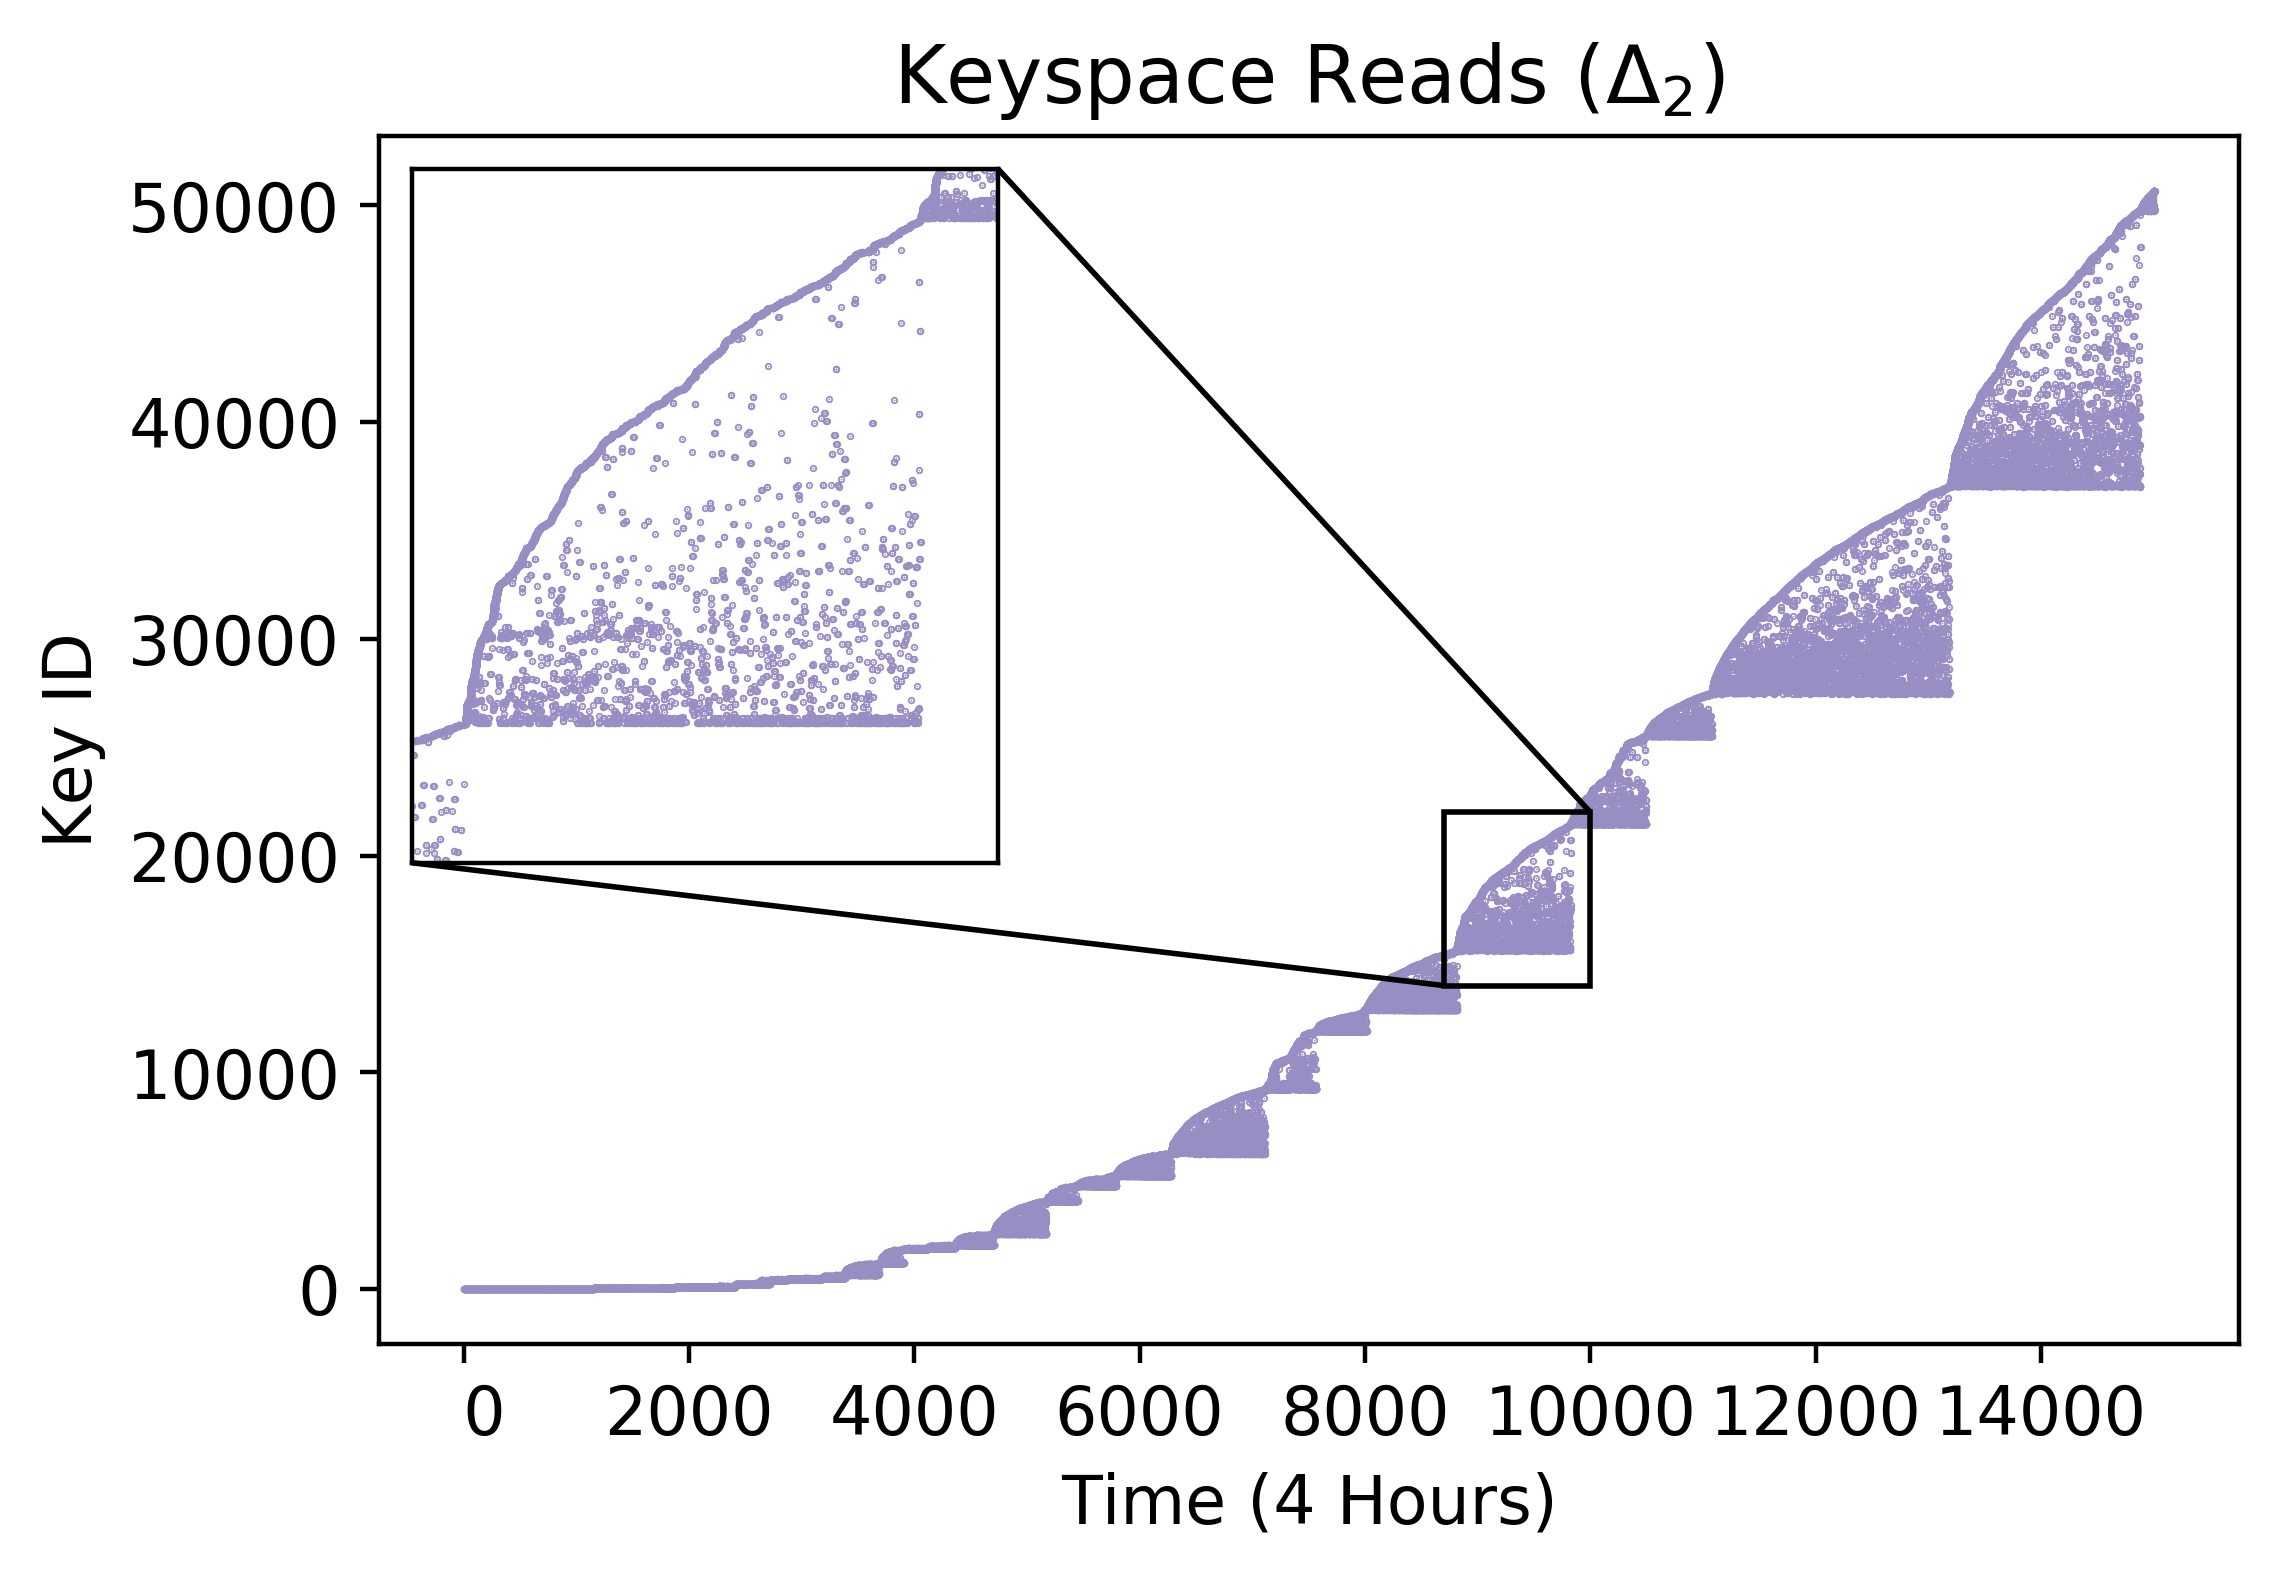
\includegraphics[height=5cm,width=0.4\textwidth]{figures/keyspace-zoomed.png}\\

  \caption{Key activity for a 4 hour run shows groups of accesses to the same
  subset of keys. Detecting these ``access regimes" leads to a more accurate cache
  management strategy.\label{fig:keyspace-zoomed}}

\end{figure}

Feeding domain-specific knowledge about the ParSplice application into a policy
leads to more a accurate cache management strategy.
Figure~\ref{fig:keyspace-zoomed} shows which keys (\(y\) axis) are accessed by
the ParSplice tasks over time (\(x\) axis). The groups of accesses to a subset
of the keys, or ``access regimes", occur because molecules are stuck in deep
trajectories. Recall that the in-memory database stores the molecules' EOM
minima, which is the smallest effective energy that a molecule observes during
its trajectory. So molecules stuck in deep trajectories explore the same minima
until they can escape to a new set of states. This exploration of the same set
of states is called a superbasin. 

Detecting these superbasins can lead to more effective cache management
strategies because the height of the keyspace accesses is ``how much" of cache
to evict and the width of the keyspace accesses is ``when" to evict values from
the cache.  The zoomed portion of Figure~\ref{fig:keyspace-zoomed} shows how a
single superbasin affects the key accesses. Moving along the \(x\) axis shows
that the number of unique keys accessed over time grows while moving along the
\(y\) axis shows that early keys are accessed more often.  Overall, superbasins
are never re-visited because the simulation only adds molecules; we can never
reach a state with less molecules. This is why keys are never re-accessed.
Despite these patterns, the following characteristics of superbasins make it
hard to detect them:

\begin{itemize}

  \item superbasin key accesses are random and there is no threshold ``minimum distance
  between key access" that indicates we have moved on to a new superbasin

  \item superbasins change immediately

  \item the number of keys a superbasin accesses differs from other superbasins

\end{itemize}

Below we describe the policies we implemented and deployed using Mantle. 

\subsection{Failed Strategies}
These techniques proliferated more knobs that obfuscated the problem. 
\begin{itemize}
  \item Statistics
  \item Calculus
  \item K-Means
  \item DBScan
  \item Anomaly Detection
\end{itemize}

\subsection{Regime Detection}

At each time step, we find the lowest ID and compare against the local minimum,
which is the smallest ID we have seen thus far. If we move left to right, the
local minimum never changes because the local minimum will start small. If we
move from right to left, the local minimum changes at each access regime.  For
points \(z\), \(y\), and \(x\), if the local minimum is the same we are in a
regime. Processing \(y\), we set the local minimum to be \(min(y, m_l)\), where
\(m_l\) is the local minimum of the previous time step of \(z\). The algorithm
incorrectly detects a regime change if the local minimum of \(y\) is lower than
local minimum of \(z\), since \(y\) may have points {\it within} \(z\); recall
that we are trying to detect the whole fan, not just the bottom edge of each
fan.

\subsection{Trajectory Length}

\subsection{Cloud Techniques: Elastic Search}

What if we re-provision resources in response to events outside the
application's control, such as a slow Lustre.

\subsection{Future work}

How Much: cache policy from past, regime detection, Belady's Min
